\documentclass[tikz,border=2pt]{standalone}
\usepackage{styles/polymer-paper-preamble}
\begin{document}
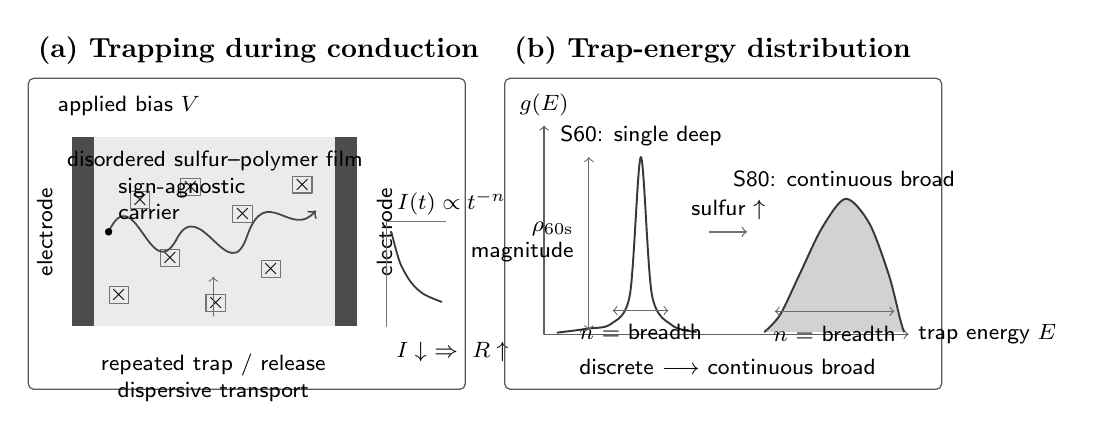
\begin{tikzpicture}[x=1cm,y=1cm, font=\sffamily\footnotesize, line cap=round, line join=round]
% Panel A: applied bias, sign-agnostic dispersive transport, and transient-current decay
\node[anchor=west,font=\bfseries] at (0,4.55) {(a) Trapping during conduction};
\draw[draw=black!65,line width=.45pt,rounded corners=2pt] (0,0.25) rectangle (5.55,4.2);
\node[anchor=west] at (0.25,3.85) {applied bias $V$};
\fill[black!70] (0.55,1.05) rectangle (0.83,3.45);
\fill[black!70] (3.90,1.05) rectangle (4.18,3.45);
\node[rotate=90,anchor=south] at (0.43,2.25) {electrode};
\node[rotate=90,anchor=north] at (4.30,2.25) {electrode};
\fill[gray!16] (0.83,1.05) rectangle (3.90,3.45);
\node[align=center] at (2.37,3.15) {disordered sulfur--polymer film};
\foreach \x/\y in {1.15/1.45,1.42/2.65,1.80/1.92,2.06/2.82,2.38/1.35,2.72/2.48,3.08/1.78,3.48/2.85} {\node[draw=black!55,inner sep=.2pt] at (\x,\y) {$\times$};}
\draw[draw=black!72,line width=.65pt,->] (1.02,2.25) .. controls (1.35,2.95) and (1.55,1.55) .. (1.88,2.15) .. controls (2.18,2.75) and (2.55,1.50) .. (2.78,2.20) .. controls (3.02,2.88) and (3.34,2.15) .. (3.65,2.52);
\fill[black] (1.02,2.25) circle (1.35pt);
\node[anchor=south west,align=left] at (1.02,2.28) {sign-agnostic\\carrier};
\node[anchor=north,align=center] at (2.35,0.82) {repeated trap / release\\dispersive transport};
\draw[->,draw=black!58] (2.35,1.18) -- (2.35,1.68);
\draw[draw=black!55,line width=.4pt] (4.55,1.05) -- (4.55,2.38) -- (5.30,2.38);
\draw[draw=black!78,line width=.65pt] plot[smooth] coordinates {(4.61,2.25) (4.72,1.86) (4.86,1.61) (5.02,1.46) (5.25,1.36)};
\node[anchor=west] at (4.56,2.62) {$I(t)\propto t^{-n}$};
\node[anchor=west,align=left] at (4.55,.72) {$I\downarrow\ \Rightarrow\ R\uparrow$};

% Panel B: discrete-to-continuous trap-energy distribution with orthogonal metrics
\node[anchor=west,font=\bfseries] at (6.05,4.55) {(b) Trap-energy distribution};
\draw[draw=black!65,line width=.45pt,rounded corners=2pt] (6.05,0.25) rectangle (11.60,4.2);
\draw[->,draw=black!62] (6.55,0.95) -- (11.18,0.95) node[anchor=west] {trap energy $E$};
\draw[->,draw=black!62] (6.55,0.95) -- (6.55,3.60) node[anchor=south] {$g(E)$};
\draw[draw=black!78,line width=.7pt] plot[smooth] coordinates {(6.72,0.97) (7.10,1.02) (7.40,1.08) (7.64,1.45) (7.78,3.20) (7.92,1.45) (8.18,1.06) (8.48,.98)};
\node[anchor=south] at (7.78,3.22) {S60: single deep};
\draw[<->,draw=black!58] (7.42,1.25) -- (8.13,1.25);
\node[anchor=north] at (7.78,1.20) {$n$ = breadth};
\draw[<->,draw=black!58] (7.12,1.00) -- (7.12,3.20);
\node[anchor=east,align=right] at (7.05,2.12) {$\rho_{60\mathrm{s}}$\\magnitude};
\draw[->,draw=black!55,line width=.5pt] (8.65,2.25) -- (9.13,2.25);
\node[anchor=south] at (8.89,2.28) {sulfur $\uparrow$};
\fill[gray!35] plot[smooth] coordinates {(9.35,.98) (9.55,1.20) (9.80,1.72) (10.08,2.30) (10.38,2.67) (10.68,2.36) (10.93,1.70) (11.07,1.15) (11.12,.98)} -- cycle;
\draw[draw=black!78,line width=.7pt] plot[smooth] coordinates {(9.35,.98) (9.55,1.20) (9.80,1.72) (10.08,2.30) (10.38,2.67) (10.68,2.36) (10.93,1.70) (11.07,1.15) (11.12,.98)};
\node[anchor=south] at (10.36,2.70) {S80: continuous broad};
\draw[<->,draw=black!58] (9.48,1.24) -- (11.00,1.24);
\node[anchor=north] at (10.24,1.18) {$n$ = breadth};
\node[align=center] at (8.88,.53) {discrete $\longrightarrow$ continuous broad};
\end{tikzpicture}
\end{document}
